\section{Definition of a 3D display}
While it is commonplace to hear about 3D display in television or smartphone advertisement nowadays, the distinction between 2D and 3D might be more difficult to settle.
\subsection{The problem}
If we take the simple definition : a 3D display is a display that can show 3D images, it is really ambiguous, because of what is supposed to be "3D". For instance, for years, video games have been advertising 3D engines and spectacular 3D graphics, even without the depth provided by what is now called 3D displays or 3D movies in cinema.
Another literal but limited definition for a 3D display would be a display that really exists in three-dimensions; one could think for instance of programmable matter and claytronics, or at least of a display that would be able to show a scene or an object from any point of view.

Hence, we have to qualify what is 3D and what it is not, in order to build a real definition.

\subsection{Parameters}
In the literature, the main idea is to relate to the human brain and body capabilities to define 3D vision (\cite{okoshi1976three}, \cite{pimenta2012comprehensive}). For instance, a big part of the "3D" feel is due to the fact of having two eyes that looks in the same direction, but from a slightly different angle, but it is not the only parameter.

The visual cues of 3D vision are separated in two families:  
\begin{itemize}
\item Physiological cues. They will relate to the capabilities of the human body.
\item Psychological cues. They will relate to the information inference capabilities of the human brain.
\end{itemize}
\subsection{Presentation of common visual cues}
Most of the visual cues on \ref{fig:visualcues} are explained in-depth in \cite{pimenta2012comprehensive}, however a short explanation is provided in the glossary for many of them.
\begin{figure}[h!]
\centering
\begin{tabular}{lr}
\begin{tabular}{|c|}
\hline
Psychological cues \\
\hline
\Gls{occlusion} \\
\Gls{linpersp} \\
\Gls{atmpersp} \\
\Gls{shading} \\
\Gls{motionparallax} \\
\Gls{kineticdepth} \\
\hline
\end{tabular} & 
\begin{tabular}{|c|}
\hline
Physiological cues \\
\hline
\Gls{stereoscopy} \\
\Gls{convergence} \\
\Gls{accomodation} \\
Retinal image size \cite{mehrabi2013making} \\
Texture gradient \cite{howard2012perceiving} \\
\hline
\end{tabular}
\end{tabular}
\caption{Common visual cues}
\label{fig:visualcues}
\end{figure}

A complete classification of the current state of the art in 3D displays using these visual cues is present in \cite{mehrabi2013making} on Table 2.

\subsection{Definition of a 3D display}
The definition retained in \cite{pimenta2012comprehensive} is the following : a 3D display is a display that uses at least one of the physiological cues. We will see that most of the displays use the stereoscopy cue, because it is the one that provides the most convincing 3D experience\cite{kaufman122006perceptual} thanks to \gls{stereopsis}.

\section{Classification of the 3D displays}
One of the main problem while trying to find a proper \gls{display} for a given application is to choose a relevant classification for the displays, that allows a choice with criterions relevant to the application.
\subsection{Criterions}
There was a lack of proper nomenclature in the literature for a long time \cite{pimenta2012comprehensive}. However, some attempts have been made to find relevant criterions that would be general enough to cover the current display techniques, but also the ones that are not yet thought of.

\subsubsection{Different classifications}
The first classification was in \cite{okoshi1976three}, and it was really based upon the different kinds of displays existing at the time: 
\begin{itemize}
\item Lens-sheet three dimensional pictures.
\item Projection-type three dimensional displays.
\item Holography.
\end{itemize}

However, it did not hold well against the emergence of new techniques, like volumetric displays for instance.

Other classifications %\cite{ref nécessaire} 
would limit themselves to only a subset of 3D displays.

Hence the need for a classification that would not base itself on the different technologies, but on criterions that would be inherent to the idea of display and human vision.

\subsubsection{Chosen classification}
In \cite{pimenta2012comprehensive}, the main idea is to classify the displays according to two axes : 

\begin{itemize}
\item The display depth (flat or deep).
\item The number of points of view from which the image can be seen (duoscopic, multiscopic, or omniscopic).
\end{itemize}

\section{In-depth presentation of some 3D display methods}
This section describes the different technologies used by manufacturers of 3D displays, and also explains some 3D visualization systems in detail. But first we will define what are stereoscopic and auto-stereoscopic displays. \\
\textbf{Stereoscopy} is the set of techniques used to reproduce a depth perception from two planar images.\\
\textbf{Autostereoscopy} is a method of image representation, either in three-dimension or stereoscopic, which requires no additional device to render the 3D effect. 


\subsection{Two-view 3D displays}
This is the category of most commercial 3D display technologies, like the common 3D TV screens or 3D movie theater technologies. The main feature of these screens, which distinguishes them from conventional screens, is their ability to display stereoscopic images : each eye of the observer will receive a different point of view.
There are multiple technologies that are able to power such screens; we will explain some. But an exhaustive list is present in \cite{mehrabi2013making}.

\subsubsection{About the time}
There are two major technologies that are in use to create a 3D effect from two image streams.
\subsubsection{Time-sequential displays}
The idea is that the images are shown one after the other, but it has two requirements : 
\begin{itemize}
\item The switching between images must be fast : a refresh rate of 48 Hz is theoretically minimal for a 24 fps movie, however research \cite{holliman2011three} shown that 58 Hz is a practical minimum.
\item Each eye must see only the images directed to it. There are multiple technologies to achieve this, passive and active.
\end{itemize}

\subsubsection{Time-parallel displays}
This is the opposite of time-sequential two-view displays. Both eyes receive a stream of images at the same time.

\subsection{Presentation of the methods}
\paragraph{Wavelength selective displays}
The most famous are the anaglyph glasses, pictured on figure \ref{fig:anaglass}. However, the result is of poor quality and unpleasant after some time.

\begin{figure}[h!]
\centering
\centering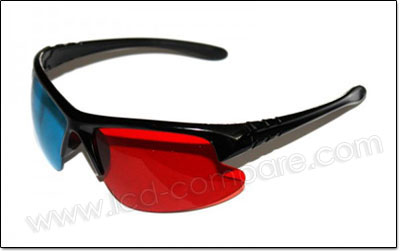
\includegraphics[width=6cm,height=40mm]{image/1.jpg}
\caption{Red/cyan colour filter 3D glasses}
\label{fig:anaglass}
\end{figure}

In this case, images are filtered by colour. The two images are superimposed and the glasses incorporate a colour filter. Each eye can only see the image intended for it, so this can be used to create a stereoscopic effect. 

This is generally used as a time-parallel method.

\paragraph{Polarized method}
\label{par:polarized}
This technique uses polarized glasses. The right lens is polarized in one direction while the left lens is polarized in the other direction, as in figure \ref{fig:polarized3D}. 

\begin{figure}[h!]
\begin{center}
\begin{minipage}{1\linewidth}
\centering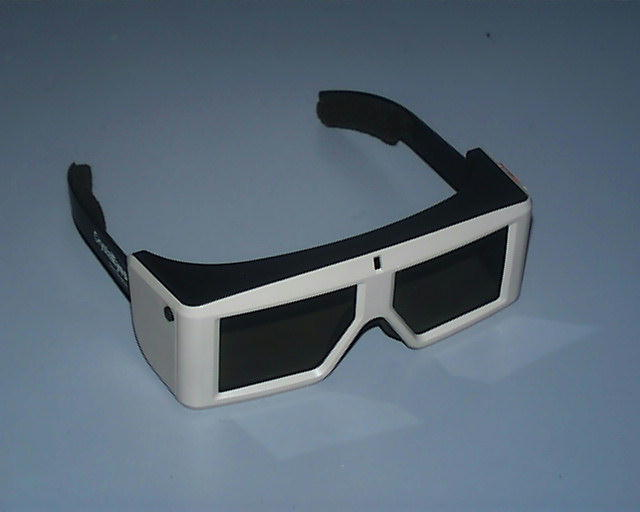
\includegraphics[width=6cm,height=30mm]{image/2.jpg}
\caption{Polarized 3D system}
\label{fig:polarized3D}
\end{minipage}
\end{center}
\end{figure}

This is not an expensive method, however the image is often less bright. It is generally used in movie theaters.

\paragraph{Active method}
This technique uses active glasses, with LCD shutters that needs to be perfectly synchronized with the screen refresh rate : one of the glass goes black while the other allow the light to pass, which allows the eyes to receive only the wanted image at the wanted time.

This method is more expensive, but reviews often said it offers a better experience.

It is a time-sequential method.

\paragraph{Multi-screen display}
This design uses multiple LCD displays, one seen in transmission and the other in reflection in a mirror, in order to change the polarization of the reflected screen.

This way, with polarized glasses, it as again possible to see with stereoscopy.

\paragraph{Auto-stereoscopy}
This technique is interesting, because no special headgear is required : the correct light information is sent directly by the screen to the eyes.

However, the viewer has to be at a precise position in front of the screen for it to work. Hence, it only works with a single person except in the case of a very large and expensive screen.

Some recent designs can for instance use reflective screens \cite{smithwick2013autostereoscopic}.

\subsection{Horizontal parallax multiview 3D displays}
Multiview or multiscopic displays are displays that can be seen from a finite number of point of view and show a different picture corresponding to this point of view.

There are two main types of technology for multiview parallax displays: either by applying a parallax barrier, or by application of a lenticular panel.

A parallax barrier is a mask of parallel black stripes that reveals the different parts of the underlying image depending on the direction of observation.

The same effect can be obtained with the lenticular sheets, which are linear networks of narrow cylindrical lenses. Both techniques are used to show a unique view of each position in the viewing area. Thus, a viewer feels the motion parallax and binocular stereo without the use of special glasses. 

\subsubsection{Lenticular Displays}
The application of a lenticular panel to deflect the rays from the pixels of the screen in order to reproduce a stereoscopic display giving the images an impression of depth.

A lenticular panel is composed of a regular grid of small spherical lenses. Each lens covers an area of several pixels of the flat screen and will divert the direction of the light emitted by the pixels covered.

As we can see on figure \ref{fig:lenticular}, each eye only sees the right or left pixels. An observer looking at a lenticular 3D screen does not see the same screen pixel between his left eye and his right eye, although both eyes see the same lenses.

With horizontal lenses, projecting changing images, the perceived image depends on the angle between the eye and the lenses.

\begin{figure}[h!]
\centering
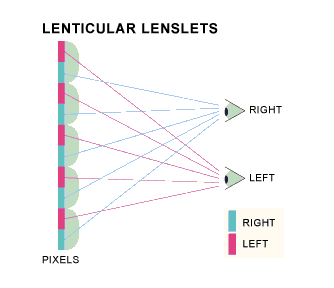
\includegraphics[width=8cm,height=5cm]{image/lentuc.png}
\caption{A lens array}

\label{fig:lenticular}
\end{figure}

\subsubsection{Parallax Barrier Displays}
Instead of lenses, multiple small masks are put in front of the pixels. The images are divided into columns of a width of one pixel.
Each mask is precisely placed so that the observer, himself set at the correct distance from the screen, views the image that corresponds to each eye. 

Thanks to the cache, an image is sent to the right eye and another in the left eye, as in figure \ref{fig:paraba}; the brain recreates the 3D picture by stereopsis.

In comparison with the lens array, we can see each spherical lens replaced by an opaque surface and a small hole in its center. Therefore, as in the case of the lens array, an observer looking at a small hole in the 3D screen does not see the same screen pixel between his left eye and his right eye: this is because the parallax barrier is not contiguous to the flat screen, but there is a distance of a few millimeters between the two panels.
\clearpage

\begin{figure}[h!]
\centering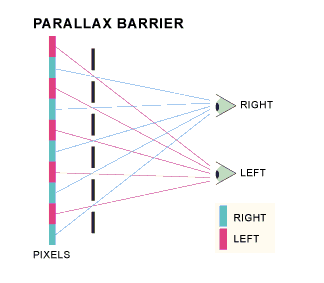
\includegraphics[width=8cm,height=5cm]{image/parallax.png}
\caption{A parallax barrier}
\label{fig:paraba}
\end{figure}

This technique provides a 3D vision without wearing glasses.

However, there are some disadvantages :
\begin{itemize}
\item It must be placed precisely over the screen, if the observer is not in a precise position, he will see superimposed images which will make the image look garbled.
\item Hence, movement is not compatible with this system, but it is very difficult for human beings to stay still for the length of a movie, for instance.
\item It does not allow visualization of stereoscopic image for multiple viewers at the same time.
\item Brightness is generally lower due to most of the light being occluded by the mask However, a recent amelioration on this technique greatly improves brightness\cite{lv2014shared}.
\end{itemize}

\subsection{Omni-view Displays}
These displays can be seen from more than a point of view and would show a correct image from any accessible point of view.

\subsubsection{Multi-projector display}
This method consists in positioning several projectors in a circle. They all display the image under a different angle. The images are projected onto a special screen. For instance, a double lenticular lens example (a spherical lens) works well, but the easiest way is to project these images on a cylindrical fog, as in figure \ref{fig:cilfog}.

Lasers can also be used : they would provide more contrast, but shapes cannot be very detailed.

\begin{figure}[h!]
\centering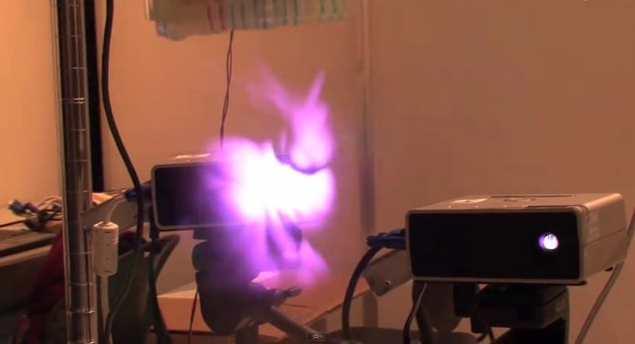
\includegraphics[width=6cm,height=4cm]{image/lapin.png}
\caption{3D multiviewpoint display}
\label{fig:cilfog}
\end{figure}

In this example, is possible to turn around the rabbit in 3 dimensions and view it from every angle.

This technique has some advantages : 
\begin{itemize}
\item There is no limit of size for the projection, which makes it good for live performance.
\end{itemize}

However, it has important requirements : 
\begin{itemize}
\item Multiple projectors are needed.
\item Headlights must be precisely aligned.
\end{itemize}

\subsubsection{Pepper's Ghost}
Pepper's ghost is an optical illusion technique used during plays, in circuses and with some magic tricks.\\
This artifice was invented in 1862 by Henry Dircks. He took advantage of an optical effect which gives the impression of a ghost appearing and vanishing in the scene.\\
In the same year, John Henry Pepper, decided to start working on illusions after going to an Henry Dircks' show. He realized that with some technique improvements, this illusion would be more cost-effective for theater renters.\\
The name of this method comes from this man because he made this effect popular.\\

The illusion is produced by glass sheets and lighting effects. The actor who plays the ghost is placed in a dark room, invisible from the audience (an hidden scene), in such a way that the public cannot directly see him\cite{Peppers-ghost}. 
The figure \ref{fig:pepperghost} explains how it works.

\begin{figure}[h!]
\centering
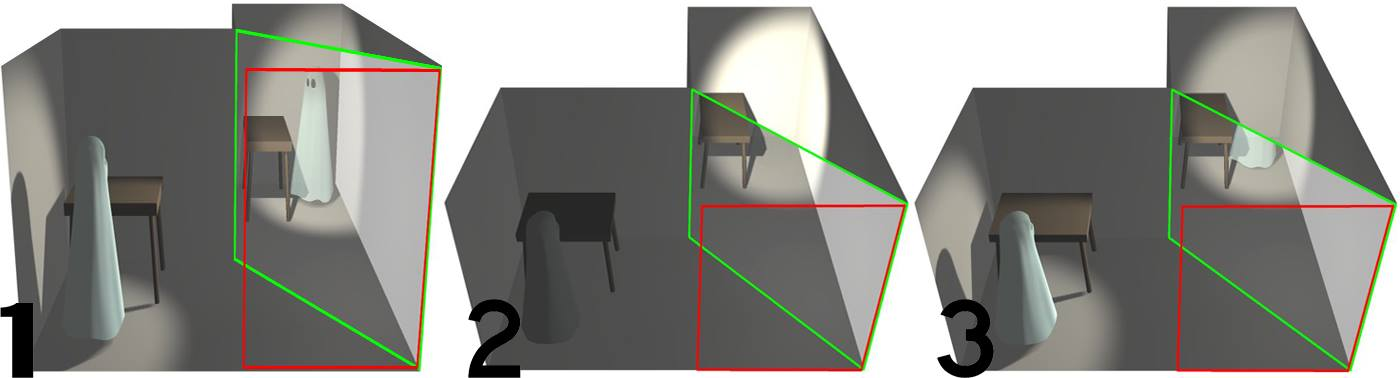
\includegraphics[width=14cm,height=4cm]{image/peppersG.jpg}
\caption{Pepper's ghost}
\label{fig:pepperghost}
\end{figure}

\begin{enumerate}
\item A viewer looking through the red rectangle sees a ghost floating next to the table. The illusion is created by a large piece of glass situated at a $45$\textdegree{} angle between the viewer and the scene (green outline). The glass reflects a room hidden from the viewer (on the left), sometimes called a "Blue Room" that is built as a mirror-image of the scene.
\item If the mirror-image room (left) is darkened, it does not reflect well in the glass. The empty room (top) is brightly lit, making it very visible to the viewer.
\item  When the lights in the mirror-image room are raised (with the empty room being dimmed slightly to compensate), the ghost appears out of nowhere.
\end{enumerate}

Nowadays, the hidden scene has been replaced by a video projector. This enables the director of the spectacle to display anything on the screen. Pepper's ghost used to be a theater-specific trick, but today digital devices revive this technique.